\taskpic{ Тело плотностью $\rho$ плавает на границе раздела двух
  жидкостей с плотностями $\rho_1$ и $\rho_2$. Найдите отношение
  объёма тела, погруженного в нижнюю жидкость $V_1$ к объёму,
  находящемуся в верхней жидкости $V_2$. }
{ 
  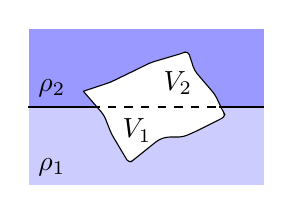
\begin{tikzpicture}
    \draw[white,fill=blue!20] (0,0) node[right=0.3cm,above,black] {$\rho_1$} rectangle (3,1);
    \draw[white,fill=blue!40] (0,1) node[right=0.3cm,above,black] {$\rho_2$} rectangle (3,2);
    \draw[decoration={random steps,segment
      length=0.3cm,amplitude=.1cm},decorate,rounded corners=.05cm,fill=white]
    (0.7,1.2) -- (1,1.3) -- (2,1.7) -- (2.5,0.9) -- (1.7,0.6) -- (1.3,0.3)
    -- (0.7,1.2);
    \draw (1.38,0.7) node {$V_1$};
    \draw (1.9,1.3) node {$V_2$};
    \draw (0,1) -- (0.8,1) (2.42,1) -- (3,1);
    \draw[dashed] (0.8,1) -- (2.42,1);
  \end{tikzpicture}
}
% ГГК, 6.17